\section{Evaluation der Theorie}
\subsection{Intro}
Dies Kapitel dient zur Evaluation der beiden Thesen.\\
Zum einen soll es möglich sein sich in Internetforen automatisch registrieren und anmelden zu können, sowie Posts passend zu Firmenpordukten aus dem Forum zu extrahieren.\\
Anderseits soll es automatisch möglich sein die Datenbankgröße des Forums durch Suchanfragen zu bestimmen, sowie eine Aussage über die Relevanz eines Forums für ein Unternehmen zu generieren.
\subsection{Evaluierungsumgebung}
Für die Evaluation der Thesen werden verschiedene Vorraussetzungen benötigt. Ein Forum, welches einen Registrierungsprozess und einen Loginprozess bereitstellt. Weiterhin muss dieses Forum die Möglichkeit bieten nach bestimmten Begriffen suchen zu können und entsprechende Treffer mit einer eindeutigen ID zurückzugeben.\\
Dazu muss das Forum zugriff auf eine Datenbankquelle haben. Diese besteht für die Dauer der Evaluation, aus einem Teil der N2O-Datenbank mit 50.000 Einträgen. Diese Einträge umfassen einen Posttitel , einen Postinhalt und eine eindeutige Weburl, die als ID benutzt wird. Die Posts sind in einer NoSQL-Datenbank, Elasticsearch, gespeichert. Diese bietet den Vorteil, das mit nur einer Anfrage an die Datenbank in Posttitel und Postinhalt nach einem bestimmten Suchwort gesucht werden kann, und die ersten Top 100 gefundenen Posts zurückgeliefert werden können.\\
Das Forum wird lokal erstellt, um eine vielzahl an Anfragen an ein im Internet verfügbares Forum zu vermeiden. Eine ordentliche Evaluierung könnte diesem Forum durch zu viel Netzwerkverkehr eventuell schaden.\\
Geschrieben werden alle Programme, die die Thesen umsetzen, mit Hilfe von JavaScript. Das Forum wird auf einem Node-Server laufen. 
\subsection{Aufbau des Forums}
Das Forum sollte einem orginalen Internetforum möglichst nahe kommen, jedoch gleichzeitig eine Umgestaltung der einzelnen Seiten für Anmelden, Registrieren und Suchen nicht allzu aufwändig machen. Dieses erlaubt ein schnelles debuggen, wenn sich das Programm nicht wie erwartet verhält. Deshalb wird sich bei dem Erstellen des Forums auf die wichtigsten Elemente konzentriert. Diese umfassen eine Login-, eine Registrierungs- und eine Suchseite.
\subsection{Registrierung im Forum}
Die häufigste Registrierungsform die man in diversen Internetforen findet bestehen aus 2 Feldern für das Passwort, 2 Feldern für die Email, einem Feld für den Nutzernamen und eine Chekbox, dass die Foren-AGB angenommen werden. Dieses wird simpel duch das folgende Codebeispiel nachgebaut.

\begin{lstlisting}[language=HTML5]
<form action="/reg" method="post">
	Nutzername: 
	<input type="text" name="fname"></br>
	Email: 
	<input type="text" name="email"></br>
	Validate Email: 
	<input type="text" name="re_email"></br>
	Password: 
	<input type="password" name="pwd"></br>
	Validate Password: 
	<input type="password" name="re_pwd"></br>
	Accept AGB:
	<input type="checkbox" name="AGB"></br>
 		 <input type="hidden" name="val1" 
            value="hiddenvalue1">
  		<input type="hidden" name="val2" 
            value="hiddenvalue2">
	<input type="submit" value="Submit">
</form>
\end{lstlisting}
\newpage

Dieses HTML erzeugt eine Registrierungsseite, die bei vielen Foren vorkommt. Nun ist es leicht zu Evaluieren, ob der Registrierungsprozess erfolgreich sein würde. Zu erwaren wäre ein POST-Request an die Toplevel Domain + Formaction mit den Postparametern fname,email,re\_email,pwd,re\_pwd,AGB , sowie den hidden Key-Value-Pairs, val1=hiddenvalue1 und val2=hiddenvalue2.\\
In die Postparameter sollten in die entsprechenden Felder, fname, email und pwd jeweils der Name, die Email und das Passwort eingetragen, sowie in den re\_email, re\_pwd jeweils die Email bestätigt und das Passwort bestätigt sein, indem sie nochmals eingetippt sind.\\
Ist der HTTP-Server gestartet und wird die Registrierungsseite analysiert und der folgenede Request an den Server gesendet :\\

\begin{lstlisting}[language=HTML5]
/reg
{ val2: 'hiddenvalue2',
  val1: 'hiddenvalue1',
  AGB: 'on',
  re_pwd: 'AjZt198#ev',
  pwd: 'AjZt198#ev',
  re_email: 'jpm96353@adiaq.com',
  email: 'jpm96353@adiaq.com',
  fname: 'Dominik' }
verification email to : jpm96353@adiaq.com
\end{lstlisting}

Zu verzeichen ist, dass sich der Client eine eigene Email angelegt hat, diese stammt von der Internetseite www.10minutemail.com.
Die Registrierungsaufforderung ging an die richtige Url des Servers, wie aus dem /reg ersichtlich ist. Weiterhin sind alle erforderlichen Parameter des Post-Requestes entsprechend ausgefüllt, und auch die Wiederholungsfelder von Email und Passwort sind korrekt ausgefüllt. Die Checkbox für die AGB ist angekreuzt worden und auch alle versteckten Input-Felder der Form mit übertragen. Insgesamt ist dieses eine gültige Registrierungsanfrage, welche der Server mit einer Validierungsemail an die angegebene Emailadresse quittiert.
\newpage
Der Client überprüft nun alle 5 Sekunden ob die Validierungsemail eingegangen ist. Sollte dieses der Fall sein wird der Link zu der Email aufgerufen, die Email analysiert und jeder darin befindliche Link aufgerufen.
\begin{lstlisting}[language=HTML5]
registered
No new emails
No new emails
No new emails
location='readmail.html?mid=KfKcm0'
https://10minutemail.net/readmail.html?mid=KfKcm0
clicked: http://localhost:12345/validateUser?user=jpm96353@adiaq.com
\end{lstlisting}
Der Validierungsversuch wird nun an den Server gesendet, der nun den Nuter als aktiven Nutzer validiert.
\begin{lstlisting}[language=HTML5]
/validateUser?user=jpm96353@adiaq.com
validate:
jpm96353@adiaq.com
\end{lstlisting}
Sollte der Registrierungsprozess nicht funktionieren, kann die Registrierungsform nachgebaut werden, gegebenfalls Änderungen an den Feldbewertungsmetriken gemacht werden und dann erneut ausprobieren, ohne Webforen zu belasten. Es gibt auch die Möglichkeit für das Programm den Registrierungsschritt zu überspringen, wenn der Nutzer schon einen Nutzeraccount per Hand angelegt hat, kann er das dem Programm über Eingabeparameter mitteilen. Anstatt sich neu zu registrieren, nutzt er nun den vorhandenen Nutzeraccount.
\newpage
\subsection{Forenlogin}
Der Forenlogin sollte bei nicht angegebenen Logindaten mit den zuvor generierten Daten ausgeführt werden, werden Daten angegeben sollten diese auch benutzt werden. Der Loginrequest sollte 3 Parameter enthalten, einmal den Nutzernamen und einmal das Passwort. Die Checkbox gibt an ob man auf der Website eingeloggt bleiben möchte, um bei einem späteren Besuch nicht nochmal die Nutzerdaten eingeben zu müssen. Das sind die gängigsten Loginformulare, die im Internet herrschen.
\begin{lstlisting}[language=HTML5]
<form action="/log" method="post">
  Nutzername: 
    <input type="text" name="fname"></br>
  Password: 
    <input type="password" name="pwd"></br>
  Eingeloggt bleiben: 
    <input type="checkbox" name="remember">
    <input type="submit" value="Submit">
</form>
\end{lstlisting}
\begin{lstlisting}[language=HTML5]
loginattempt: 
{fname:'Dominik',
 remember: 'on',
 pwd:'AjZt198#ev'}
\end{lstlisting}
Es ist zu sehen, das alle erforderlichen Daten korrekt ausgefüllt wurden. Auch wenn die Loginform Usernamen und Email abfragen sollte, wird ein valider Loginrequest abgesendet.
\begin{lstlisting}[language=HTML5]
loginattempt:
{email: 'jpm96353@adiaq.com',
 fname: 'Dominik',
 remember: 'on',
 pwd: 'AjZt198#ev'}
\end{lstlisting}
Auch etwaige versteckte Input-Felder werden korrekt gefunden und die Key-Value Paare in dem POST-Request mit übergeben.
\begin{lstlisting}[language=HTML5]
loginattempt:
{email: 'jpm96353@adiaq.com',
 fname: 'Dominik',
 remember: 'on',
 pwd: 'AjZt198#ev',
 hiddenvalue: 'v1'}
\end{lstlisting}
Alle nachgebauten Loginseiten diverser im Internet gefundenen Seiten wurden im händischen Test erfolgreich ausgefüllt und die zu erwartende Loginanfrage an den Server gesendet.\\
Es ist programmatisch möglich sich in Foren automatisch zu registrieren und anzumelden. Um die erste Therorie vollständig zu evaluieren müssen naach dem Loginvorgang nun noch relevante Posts zu den jeweiligen Firmenprodukten aus dem Forum extrahiert werden.\\
Hierzu werden in Internetforen die Nutzer, die sich gerade angemeldet haben, auf die Hauptseite des Forums verwiesen. Damit der Browser das realiesiert, wird in der Antwort des Servers nach dem erfolgreichen anmelden, ein Statuscode 302 gesendet. Dieser zeigt an, das der Browser eine andere Url ohne das Zutun des Nutzers laden soll. Die Url steht im Location-Header der Antwort. Dieses muss programmatisch realisiert werden, da sonst, ohne den Redirect, bei einer Analyse des HTML Quellcodes keine Suchform gefunden werden könnte, da immer die vorherige, also die Login-Seite anlaysiert werden würde.\\
Der Server antwortet auf eine erfolgreiche Loginanfrage mit einem Redirect.
\begin{lstlisting}[language=HTML5]
successfull login from: jpm96353@adiaq.com
send 302 to redirect to /main
/main
\end{lstlisting}

Der Client schaut bei jeder Anfrage an den Server ob der Statuscode sich von 200 (OK) unterscheidet. Sollte es wie in diesem Fall ein 302 (Redirect) sein, wird automatisch die neue Url mit einem Get-Request nachgeladen, damit das neue HTML analysiert werden kann im nächsten Schritt.
\newpage


\subsection{Suchen im Forum}
\begin{lstlisting}[language=HTML5]
http://localhost:12345/log
{ email: 'jpm96353@adiaq.com',
  fname: 'Dominik',
  pwd: 'AjZt198#ev',
  hiddenvalue: 'v1' }
redirected
redirecturl: /main
\end{lstlisting}


Der Client erkennt automatisch das er auf eine andere Seite verwiesen wurde und läd diese. Dieses ist daran zu erkennen, dass das HTML was im nächsten Schritt analysiert wird nicht mehr das Login-HTML ist.

\begin{lstlisting}[language=HTML5]
<form accept-charset="UTF-8" action="/search" class="js-site-search-form" data-global-search-url="/search" data-repo-search-url="" method="get">
	<div style="margin:0;padding:0;display:inline">
	<input name="utf8" type="hidden" value="true"></div>
  <label class="js-chromeless-input-container form-control">
    <input type="text" class="js-site-search-focus  chromeless-input" data-hotkey="s" name="q" placeholder="Search OwnForum" data-global-scope-placeholder="Search OwnForum" data-repo-scope-placeholder="Search" tabindex="1" autocapitalize="off">
  </label>
</form>
\end{lstlisting}

Dieses HTML wird nach einer Suchform durchsucht. Diese befindet sich meist ein einer Get-Form. Da der Request ein get Request ist wird das Suchwort in der Url codiert. Der Name des Key-Value-Paares, welches für die Übermittelung zuständig ist, wird aus den Input-Feldern in der Form generiert. Dieses Attribut hat meist in den Namen `q` oder `search`. Der Client findet diese Suchform und sendet die Suchanfrage an den Server.

\begin{lstlisting}[language=HTML5]
{ action: '/search', name: 'q' }
\end{lstlisting}

Auf dem Server geht eine valide Suchanfrage ein.

\begin{lstlisting}[language=HTML5]
/search?q=CRM
/search?q=LVM
/search?q=HCM
/search?q=ECOM
\end{lstlisting}

Diese Suchwörter werden in dem Forum gesucht. Sollte das Suchwort in dem Titel oder dem Postcontent vorkommen, wird der Link zu diesem Post zurückgegeben. Dieser Link ist in dem Testforum eine eindeutige ID. Es ist anzunehmen das die Links eine eindeutige ID für jeden Post darstellen, da sie auf genau eine feste Internetadresse verweisen. So wie in einem Internetforum werden pro Suchwort die ersten 20 Treffer zu diesem Suchwort auf einer HTML zusammengefasst und an den Client ausgeliefert. Zu erwarten ist, dass der Client alle Links speichert und vermerkt wie oft der Link bei unterschiedlichen Suchworten von dem Forum zurückgegeben wurde. Dazu wird das HTML nach allen vorkommenden Links durchsucht. Des weiteren sollten Links die in mehr als der Hälfte der Suchanfragen wiedergegeben werden, da es sich hierbei meist um statische links handelt wie neuste Posts oder Links in den Navigationsleisten, entfernt werden.

\begin{lstlisting}[language=JavaScript]
dispatcher.onGet("/search", function(req, res) {
    res.writeHead(200, {'Content-Type': 'text/html'})
    var results = searchDataBaseForWord(req.params.q)
    .then(function(results){
        if(results.length > 0){
            var temp = ''
        for (var i = results.length - 1; i >= 0; i--) {
            temp += '<a href="/'+ results[i] +'">Link</a>'
            temp += '</br>'
        }
            temp +='<a href="/shouldberemovedLink">REMOVELINK</a>'
            temp += '</br>'
            res.write(temp)
        }else{
            var temp = ''
            temp +='<a href="/shouldberemovedLink">REMOVELINK</a>'
            temp += '</br>'
            temp += "<h1> No valid Data found </h1>"
            res.write(temp)
        }
        res.end()    
    })  
})
\end{lstlisting}

Hier wird für jede Suchanfrage das HTML zusammgebaut, dass die Links zu den jeweiligen passenden Dokumenten enthält.
Auch ein statischer Link wird plaziert, welcher dann von dem Client entfernt werden sollte, da er in mehr als der Hälfte der Anfragen vorhanden ist.

\begin{lstlisting}[language=HTML5]
/search?q=besiege
/search?q=briar
/search?q=individuals
/search?q=evacuate
/search?q=steals
/search?q=detrimental
/search?q=untimely
/search?q=bestir
/search?q=graphical
/search?q=revelation
\end{lstlisting}

\begin{lstlisting}[language=HTML5]
{"href=\"/g-1814892-S-5993338243263848452\"":1,
"href=\"/g-1850237-S-6005730948694503428\"":1,
"href=\"/g-115178-S-5999229826848821253\"":1,
"href=\"/g-66325-S-6001320511865446402\"":1,
"href=\"/g-66325-S-6003599070168440836\"":1,
"href=\"/g-54723-S-5999922118567956482\"":1}
\end{lstlisting}

Bei 10 Suchanfragen an die Datenbank, mit zufälligen englischen Wörtern wurden 6 Dokumente in der Testdatenbank gefunden. Keines wurde doppelt getroffen und der statische Link wurde entfernt. Die verbleibenden Links können nun mit einem GET-Request an den entsprechenden Link herruntergeladen und indexiert werden.

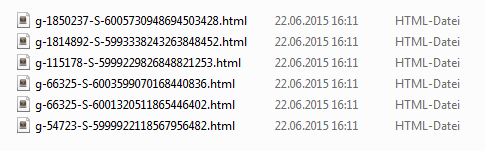
\includegraphics{./images/postdownload.png}

Es wurden erfolgreich die 6 Dokumente des Forums herruntergeladen, die das Forum auf die 10 Suchanfragen ausgeliefert hat.
Damit ist gezeigt, das es möglich ist sich automatisch in Foren zu registrieren , einzuloggen und nach bestimmten Firmenspezifischen Schlagworten für Produkte zu suchen.

\subsection{Evaluation Theorie 2}

Es geht darum zu evaluieren, ob eine Vorhersage darüber zu treffen, wie groß eine Forendatenbank ist und wie relevant dieses Forum für ein jeweiliges Unternehmen ist, erfüllbar ist.

Dazu wird zunächst die Datenbankgröße bestimmt wie in Kapitel [] beschrieben. Dafür wurde die Testdatenbank in 3 Segemente geteilt. Segement 1 enthält nur Posts aus Forum 1, Segement 2 nur aus Forum 2 und Segement 3 nur Posts aus Forum 3. 
Segement 1 und 2 beinhalten englische Posts, wohingegen Segement 3 meist deutsche Posts enthält. Die Postanzahl aller 3 Segemente ist bekannt. Um eine realistische Einschätzung zu erhalten, wie zuverlässig die Vorhersage der Gesamtdatenbankgröße ist, wurde der Test für jedes Segement 3 mal wiederholt. Ein Testdurchlauf besteht aus 3 mal 500 zufälligen Wörtern die an die Datenbank in der passenden Sprache gesendet werden. Die ermitteltelten Datenbankgrößen nach 500 Wörtern werden addiert und durch die Gesamtanzahl der Testläufe dividiert und danach mit der bekannten Gesamtanzahl der Posts in dem Datenbanksegment verglichen.

\begin{tabular}{ | p{3cm} | p{3cm} | p{3cm}| p{3cm} |}
\hline
Durchlauf & Anzahl Dok in S1 & Anzahl Dok in S2 & Anzahl Dok in S3 \\ \hline
1 & 12572  & 18374 & 8079 \\ \hline
2 & 10400 & 21155 & 7896 \\ \hline
3 & 15017 & 20952 & 8343  \\ \hline
Arith. Mittel & 12663 & 20160 & 8016 \\ \hline
Fehler & +4\% & -5\% & -1\% \\ \hline
\end{tabular}

Der Fehler beträgt maximal 5\% , dieses bestätigten die zwei weiteren Testdurchläufe. Damit ist eine Vorraussage einer Forendatenbank bis auf 10\% Differenz genau möglich sein.\\

Im nächsten Schritt sollen die einzelnen Produkte in dem Forum gesucht werden. Dazu werden wie in Kapitel[] brieben beschreibende Wörter für jedes einzelnde Produkt generiert. Diese Keywords werden gesucht und die Datenbankgröße aufgrund des Verhältnisses zwischen überlappenden und einzigartigen Dokumenten, wie in Kapitel[] beschreiben, berechnet. Die Datenbank die zu Testzwecken verwedet wurde enthält 22000 Posts.\\

\begin{tabular}{ | p{3cm} | l |}
\hline
Produkt & Anzahl der Dokumente in DB \\ \hline
CRM & 2386 \\ \hline
HCM & 3138 \\ \hline
ECOM & 3641  \\ \hline
LVM & 1769 \\ \hline
\end{tabular}

Der Rest der Posts konnte keinem Produkt eindeutig zugeordnet werden.

\begin{tabular}{ | p{3cm} | l | l |}
\hline
Produkt & Berechnete Anzahl der Dokumente in DB & Fehler\\ \hline
CRM & 3800 & +59 \%\\ \hline
HCM & 9668 & +338 \% \\ \hline
ECOM & 10604  & +265 \%\\ \hline
LVM & 39541 & +2235 \%\\ \hline
\end{tabular}

Zu verzeichnen ist das die Größe der einzelnen Produktkategorien maßlos überschätzt wurde. Deshalb wird zur Ergebnisverbesserung ein zusätzlicher Schritt eingefügt. Es werden wie bisher die Keywords zu den jeweiligen Produkten im Forum gesucht, jedoch bevor der Post zur Berechnung des Gesamtcorpus beiträgt, durch einen Klassifizierungsservice analysiert. Dieser bestimmt aus einem gegebenen Text, auf Grundlage der selben Broschüren, die zur Berechnung der tfidf- Keywords verwendet werden, welchem Produkt der Post am ehesten entspricht.

\begin{lstlisting}[language=HTML5]
http://192.168.42.54:9001/predictions?text=Hi, I want to by an CRM product
\end{lstlisting}

\begin{lstlisting}[language=HTML5]
{
   "product": [
        {
            "product": "CRM",
            "prob": 0.9999979024787202
        },
        {
            "product": "ECOM",
            "prob": 0.0000020975212798552666
        },
        {
            "product": "LVM",
            "prob": 3.0982005787342066e-25
        },
        {
            "product": "None",
            "prob": 2.2462124385020632e-66
        },
        {
            "product": "HCM",
            "prob": 1.5018464896178129e-218
        }
    ]
}
\end{lstlisting}

Dieser Post würde als CRM - Post richtig eingestuft werden. Wenn gerade die CRM - Froendatenbankgröße berechnet werden sollte, wird dieser Post mit in die Berechnung einfließen. Alle Post die als nicht CRM - Posts eingestuft werden werden in dieser speziefischen Ermittlung nicht betrachtet.\\
Mit maximal 100 generierten Keywords gewichtet nach der höchsten tfIdf werden folgende Resultate erricht.

\begin{tabular}{ | p{3cm} | l | l |}
\hline
Produkt & Berechnete Anzahl der Dokumente in DB & Fehler \\ \hline
CRM & 2270 & -5\% \\ \hline
HCM & 2730 & -14 \% \\ \hline
ECOM & 4388 & +17\% \\ \hline
LVM & 1670 & -5\% \\ \hline
\end{tabular}

Ein Fehler von maximal 20\% mit nur maximal 100 Suchanfragen ist eine zufreidenstellende Größe. Aus der Datenbankgröße und den spezifischen Produktdatenbankgrößen lässt sich sagen ob das Forum zum Verkauf eines Produktes geeignet ist oder nicht.